\documentclass[a4paper,12pt]{article}
\usepackage[ngerman]{babel}
\usepackage{ucs}
\usepackage{multirow}
\usepackage{xltxtra}
\usepackage[utf8x]{inputenc}
\usepackage{fontspec}
\usepackage[automark]{scrpage2}
\usepackage{eurosym}
\usepackage{graphicx}
\usepackage[paper=a4paper,left=25mm,right=25mm,top=25mm,bottom=25mm]{geometry}
\pagestyle{scrheadings}
\setmainfont[Mapping=tex-text]{Liberation Serif}
\clearscrheadfoot
\begin{document}
\ohead{Regelstand: \today}
\title{Regeln Jousting Challenge 2018}

 \begin{center}

\includegraphics[width=0.5\textwidth]{logo.png}

\huge                      % Schriftgröße einstellen
\bfseries                   % Fettdruck einschalten
Regeln Jousting Challenge 2020
  \end{center}
Inhaltliche Änderungen im Vergleich zu den Regeln von 2018 sind \textbf{fett} markiert. Im Zweifel ist die Interpretation der Regeln durch die Schiedsrichter bindend.
\section{Aufgabe}
Baue und programmiere einen Linienfolger, der einen Ritter mitführen kann
(gehalten von einem Magneten auf einer Metallplatte), welcher in einem
Lanzenstechen (sog. Tjost) den gegnerischen Ritter mithilfe einer
Lanze zu Boden werfen kann.
\section{Wer kann teilnehmen?}
Teams von \emph{2 bis 4 Spielern} in \emph{folgender Altersgruppe}:
\begin{itemize}
	\item Altersgruppe 1 (Middle School): 10-13 Jahre
\end{itemize}
\section{Materialanforderungen}
Autonomer Roboter basierend auf jeglicher Plattform, der maximal  \euro{ 1500} kostet und den folgenden
Designanforderungen, die beim \emph{Check-In überprüft werden}, entspricht:
\begin{itemize}
\item Der Roboter kann ein Linienfolgerprogramm am Beispiel einer Jousting-Strecke (vom Start entlang der Kurve
bis zur 100 Punkte Linie) vorführen.
\item Die Ritterbefestigungsstruktur (Marmeladenglassdeckel) kann mit jedem nicht-ferromagnetischen Material
befestigt werden, darf allerdings dem Ritter keinen Halt (außer durch den bereitgestellten Magneten)
gewähren.
\item Die Ritterbefestigungsstruktur darf maximal eine Höhe von 10 cm über dem Boden haben und sich maximal 10 cm vor dem Roboter befinden.
\item Die Flasche wird weder durch zusätzliche Befestigung unterstützt noch dürfen sich Teile des Roboters über der Metallplatte oder direkt um die Flasche herum befinden.
\item Der Ritter ist mit einem rundem Knopfmagneten mit einer Haftkraft von 800g an der Metallplatte befestigt.
\item Es dürfen sich keine weiteren Magneten innerhalb oder außerhalb des Ritters befinden.
\item Es muss ein Sensor zum Erkennen und Folgen der Linie verwendet werden.
\item Während der eigentlichen Wettbewerbs muss der offizielle Ritter des jeweiligen Jahres verwendet werden.
Dieser wird am Track bereitgestellt. Dies gilt ebenso für den Marmeladenglasdeckel, den Magneten und die
Lanze.
\item Das Volumen des Roboter darf 65030 cm$^{3}$ nicht überschreiten.
\end{itemize}
\section{Spielregeln}
\begin{itemize}
	\item Ein Linienfolgerprogramm muss den Roboter steuern.
	
	\item Während eines Duells sind maximal 5 Durchläufe erlaubt um den gegnerischen Ritter herunterzustoßen.
	\item Wenn 5 Durchläufe erfolglos durchlaufen sind, gilt das Duell als unentschieden.
	\item Wenn beide Ritter zu Boden fallen, gilt der Ritter, welcher lt. Punktrichter zuerst den Boden berührt als
	Verlierer.
	\item Nur die Lanze darf den Ritter herunterwerfen. Sollte der Ritter durch etwas anderes heruntergeworfen werfen,
	so wird mit dem nächsten Durchgang fortgefahren (außer es handelt sich um den 5. Durchgang).
	\item \emph{Nur} die Lanze darf die Mittellinie des Tracks überqueren (\textasciitilde13 cm von den jeweiligen 2 parallelen Linien entfernt).
	\item Die erreichte Punktezahl vermindert sich nach jedem erfolglosen Durchgang um 10\%. Es gibt maximal 5 Durchgänge.
\end{itemize}
\section{Spielfeld}
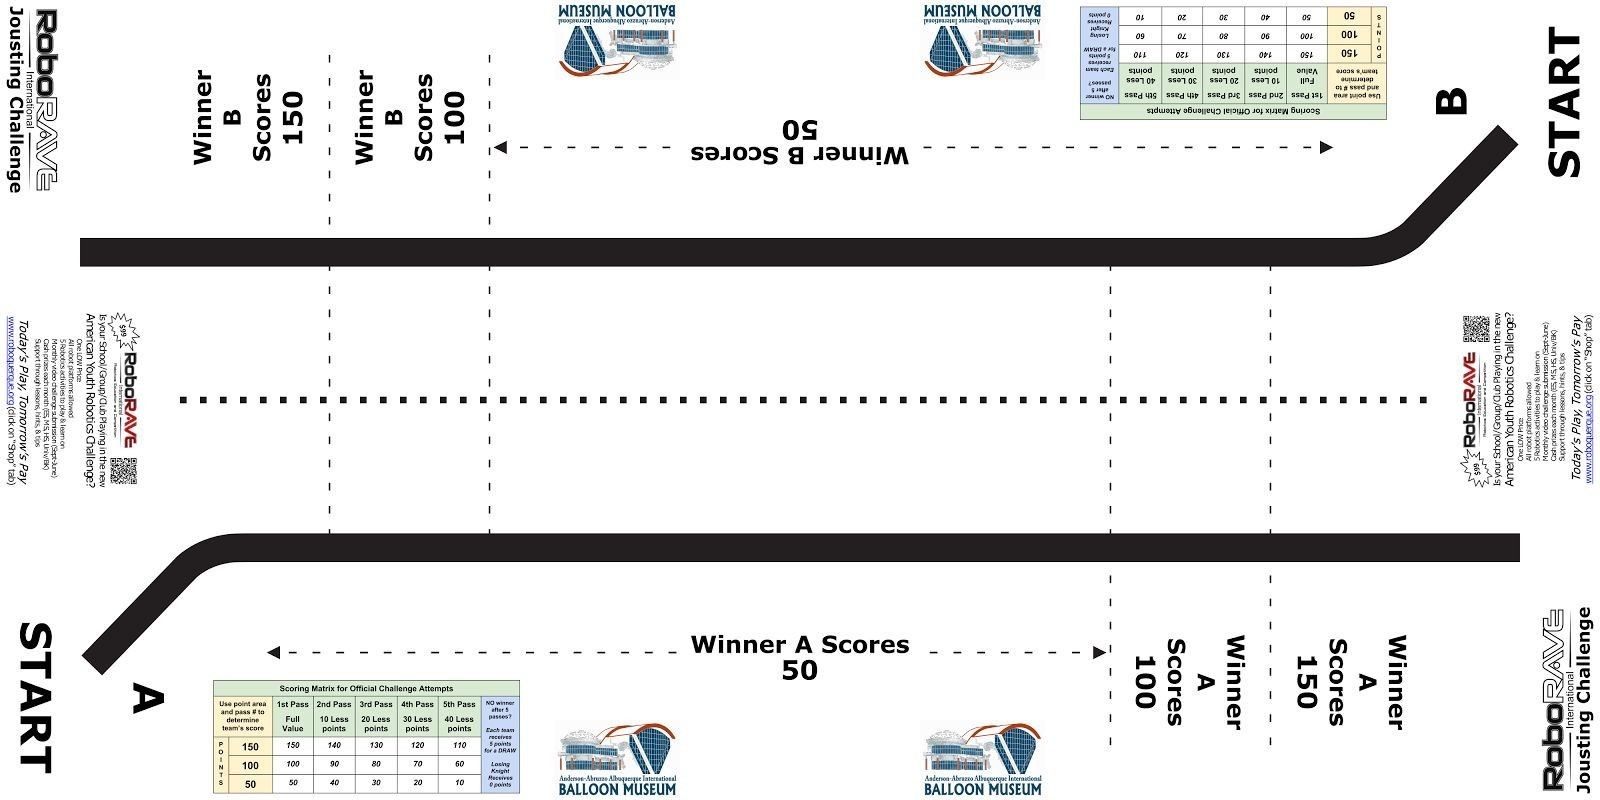
\includegraphics[width=1\textwidth]{track.png}
\begin{itemize}
	\item Zwei parallele ungefähr 2,5 cm breite Linien auf weißer PVC-Plane.
	\item Jede Linie hat zu Beginn eine leichte Kurve.
	\item Ein Meterstab \emph{kann durch die Schiedsrichter} unter der Plane entlang der Mittellinie als Schranke (sog. "Tilt") platziert werden.
	\item Es gibt 3 Scoringzonen: 150 Punkte (bis ungefähr \textasciitilde15 cm vom Start); 100 Punkte (\textasciitilde15 cm bis \textasciitilde30 cm vom
	Start); 50 Punkte (\textasciitilde30 cm bis \textasciitilde90 cm vom Start).
\end{itemize}
\section{Wertungszeitraum}
\par Die Art der Wertung der einzelnen Ergebnisse im Bezug auf den gesamten Wettbewerb wird am ersten Wettbewerbstag von den Schiedsrichtern bekanntgegeben. Änderungen der Wertungsmodalitäten bleiben den Schiedsrichtern vorbehalten.
\section{Punktevergabe}
\begin{itemize}
\item Wenn ein Roboter den gegnerischen Ritter mit der Lanze herunterstößt, ist dies der Gewinner und er erhält die unten angegebene Punktzahl.
\item Volle Punktzahl wird \emph{nur} gewährt, wenn einer der Ritter bereits im \emph{ersten} der 5 Durchläufe zu Boden geworfen
wird. Jeder weitere Durchlauf mindert die Punktezahl \emph{(siehe Tabelle)}.
\item Höhere Punktezahlen werden erzielt, je näher das Herunterwerfen an der Startposition gelingt.
\item Wenn der Ritter (\emph{nicht die Lanze}) zwischen 2 Punktebereichen liegt, zählt die höhere Punktezahl.
\item Definition: Durchlauf – ein gegenseitiger Versuch wurde unternommen den Ritter herunterzustoßen,
jedoch wurde keiner der Ritter heruntergeworfen.
\item Jedes Team hat 5 Durchläufe um den gegnerischen Ritter herunterzuwerfen.
Gibt es nach 5 Durchläufen keinen Gewinner bekommt jedes Team 5 Punkte.
\item Der Verlierer erhält 0 Punkte.
\end{itemize}
\section{Punktetabelle}
\begin{center}
\begin{tabular}{|c|c|c|c|c|c|} \hline
	\multirow{2}*{Zone} & 1. Durchlauf & 2. Durchlauf & 3. Durchlauf & 4. Durchlauf & 5. Durchlauf \\
	 & 100\% & 90\% & 80\% & 70\% & 60\% \\ \hline
	150 & 150 & 135 & 120 & 105 & 90 \\ \hline
	100 & 100 & 90 & 80 & 70 & 60 \\ \hline
	50 & 50 & 45 & 40 & 35 & 30 \\ \hline
\end{tabular}
\end{center}
\end{document}
